\documentclass{article}
\usepackage[utf8]{inputenc}
\usepackage[spanish]{babel}
\usepackage{listings}
\usepackage{graphicx}
\graphicspath{ {Pictures/} }
\usepackage{cite}

\begin{document}

\begin{titlepage}
    \begin{center}
        \vspace*{1cm}
            
        \Huge
        \textbf{Proyecto investigativo}
        
            
        \vspace{0.5cm}
        \LARGE
        Taller nociones de la memoria del computador
            
        \vspace{1.5cm}
            
        \textbf{Luis Fernando Torres Torres}
        
        \vspace{4cm}
            
        \textbf{PhD. Augusto Salazar Jiménez}
            
        \vfill
            
        \vspace{0.8cm}
            
        \Large
        Despartamento de Ingeniería Electrónica y Telecomunicaciones\\
        Universidad de Antioquia\\
        Medellín\\
        Septiembre de 2020
            
    \end{center}
\end{titlepage}

\tableofcontents%Tabla de contenidos 

\newpage

\section{Introducción}\label{intro}
Uno de los componentes más importantes dentro de la computación es la memoria, la cual está estrechamente relacionada con el concepto de almacenamiento de información y datos que contienen todos los programas. En este documento se introduce de manera clara y sencilla, ciertos conceptos que son de vital importancia para entender la definición, el funcionamiento y tipos de memoria que usa el computador para realizar cualquier proceso o tarea.

\section{Sección de contenido}
\subsection{¿Qué es la memoria del computador?} \label{contenido}
La memoria del computador sin lugar a duda cumple un papel muy importante dentro de la computación y su funcionamiento, ya que es aquel componente que se encarga de almacenar de manera temporal toda la información relevante y necesaria que va a ser procesada o usada en dicho computador.\cite{augusto}\\

La memoria almacena toda la información en grupos de bits que se denominan palabras, es decir conjunto de números 1 y 0 que puede representar un número, un carácter, una cadena de texto o cualquier tipo de información. La capacidad de las memorias en las computadoras comerciales de hoy en día se da a conocer en la cantidad de bytes que pueden almacenar. \cite{arquitectura}\\

Por otra parte el funcionamiento de una memoria tiene unas características importantes que clasifica los diferentes tipos de memoria tal como lo son la localización, la capacidad de almacenamiento, el método de acceso, la organización de los datos en una memoria, el tiempo de acceso y velocidad, entre otros.\\


Es importante reconocer que tipo de memoria usar para una tarea específica, por lo que dependiendo de sus características, es o no útil para cierto tipo de memoria como se verá en la sección \ref{tipos}. Para mayor entendimiento y esclarecer mejor el concepto de que es una memoria, es importante hablar de las características que clasifica una memoria.


\begin{itemize}
    \item \textbf{Localización de la memoria}: Esta característica hace referencia básicamente al lugar donde está posicionada la memoria dentro del computador, la cual puede estar dentro del procesador como lo es el caso de los registros y memoria caché, memoria interna como la memoria RAM, y memoria externa como lo es el disco duro o unidades ópticas.
        
    \item \textbf{Capacidad de la memoria}:Hace referencia a la capacidad de almacenamiento o a la cantidad de información que una memoria puede acumular. La unidad de información que se usa para medir esta capacidad es el byte. \cite{arquitectura}
    
    \item \textbf{Tiempo de acceso y velocidad}:Cada tipo de memoria, tiene un tiempo de acceso a sus datos, en el caso de una memoria de acceso aleatorio como la memoria RAM (la cual se explica en la sección \ref{tipos}), es el tiempo que transcurre desde que la dirección de memoria deseada se hace visible ante los circuitos de dicha memoria hasta que el dato esta almacenado, en el caso de las de acceso no aleatorio, se considera el tiempo de acceso como aquel tiempo necesario para realizar la escritura o lectura dentro de sí. Por otra parte, la velocidad de transferencia hace referencia al tiempo que transcurre entre leer y escribir información o algún dato en la memoria. \cite{arquitectura}

    
    \item \textbf {Métodos de acceso}: Hace referencia a el método que cada tipo tiene memoria tiene para acceder a las posiciones, como por ejemplo secuencial, el cual se accede desde la última posición que se ha accedido, y continua la búsqueda en orden hasta llegar a la posición deseada(ver figura \ref{vs2}), otro método es el directo, donde la memoria se divide en bloques y dentro de cada bloque se realiza un acceso secuencial hasta llegar a la posición deseada, luego está el método aleatorio, en el cual la memoria se organiza como un vector, donde cada elemento tiene una única dirección y se realiza la búsqueda de manera aleatoria(ver figura \ref{vs2}), y por último el método asociativo, donde el acceso se realiza no con la dirección de la memoria si no más bien con el contenido deseado, es decir en este método se especifica el valor a buscar y él compara el contenido de cada posición de la memoria con el contenido deseado. \cite{arquitectura}\\
    
    \begin{figure}[h]
    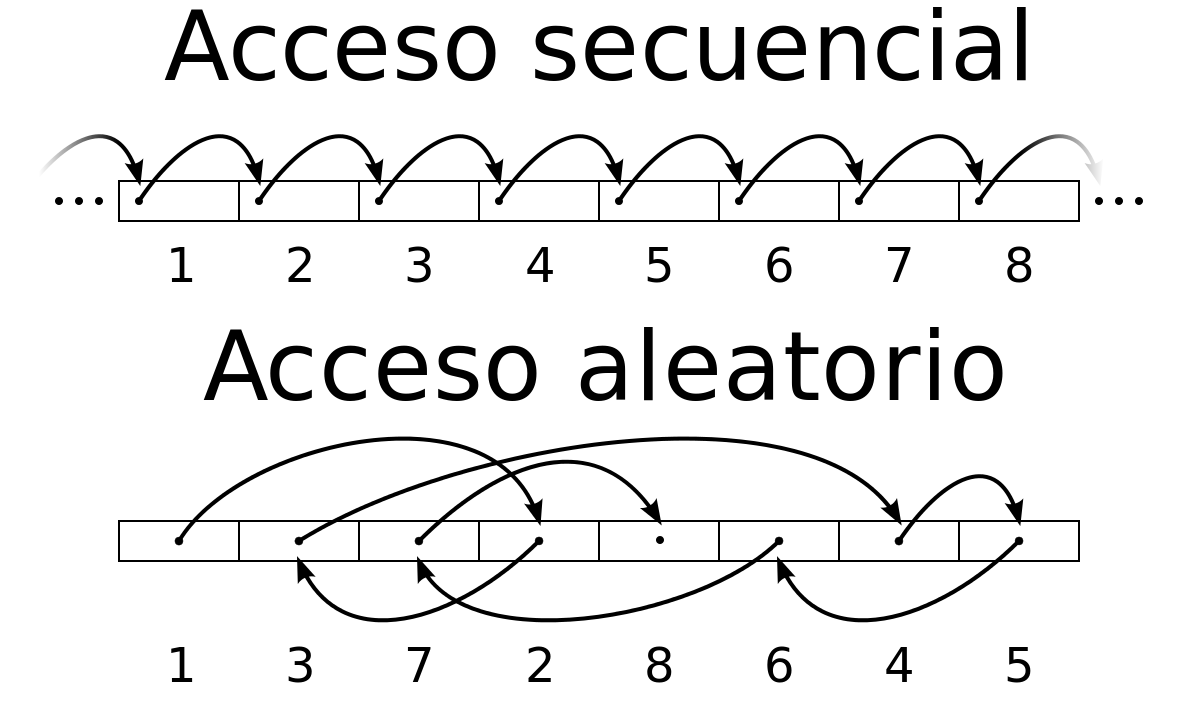
\includegraphics[width=7cm]{accesos.png}
    \centering
    \caption{Acceso secuencial vs aleatorio}
    \label{vs2}
    \end{figure}


    \item \textbf{Organización de los datos en una memoria}: Esta característica se enfoca en él como se organizan los datos de una memoria, lo cual puede darse principalmente de 2 maneras, la primera, es por medio de una unidad conocida como palabra de memoria, donde su tamaño se especia en bytes, y la otra manera es por medio de la unidad de direccionamiento, donde cada sección de la memoria se le asigna un dato con una dirección específica, y al mismo tiempo se especifica el tamaño de cada sección de dicha memoria. \cite{arquitectura}
    
\end{itemize}  

\subsection{Tipos de memoria.} \label{tipos}%Explicar usos de cada memoria

En una computadora existen diferentes tipos de memoria cada una con tareas específicas, esto con el fin de realizar de manera más eficiente y rápida el proceso, búsqueda y utilización de recursos. Dentro de esto se encuentran los siguientes tipos de memoria:

\subsubsection{Memoria ROM}
La memoria ROM (Read Only Memory - Memoria de Sólo Lectura) \cite{augusto}, es conocida como memoria no volátil ya que la información contenida en ella
no es borrable una vez se apague el dispositivo electrónico, en este vital componente se almacenan programas firmware, es decir, programas como el
sistema operativo, intérpretes o compiladores de lenguajes, y otros programas que no necesitan ser modificados actualizados, o alterados constantemente \cite{memorias}, ya que como su nombre lo indica, esta unidad solo posee la operación de lectura, no tiene posibilidad de escritura.
La memoria ROM se encuentra instalada en la tarjeta madre “motherboard” lugar donde se encuentra la información básica del equipo, llamada “BIOS.”



\subsubsection{Memoria caché}
La memoria caché, es un componente que se caracteriza principalmente por su alta velocidad de acceso, en orden de jerarquía es la memoria más rápida, pero a su vez tiene poca capacidad de almacenamiento para datos e información. En esta memoria se almacenan temporalmente los datos que son usados con mayor frecuencia, para así lograr tener un acceso rápido, casi inmediato\cite{arquitectura}. Dicha memoria caché está directamente interconectada con el microprocesador y se divide en tres niveles (levels en inglés) L1, L2 y L3. \cite{augusto}, donde a medida que el nivel va aumentando su capacidad de almacenamiento va aumentado también y su velocidad de acceso va disminuyendo, es decir la memoria más veloz, pero con menos capacidad es L1, y por el contrario la menos veloz, pero con mayor almacenamiento la memoria caché L3.


\subsubsection{Memoria RAM}
La memoria RAM (Random Access Memory - memoria de Acceso Aleatorio), es sin duda la memoria más conocida e importante del computador, recibe dicho nombre, dado a que está divida en celdas de memoria, donde se almacenan temporalmente cada uno de los bits o pulsos eléctricos que contienen toda la información con la que trabaja el microprocesador. \cite{augusto}\\

La memoria RAM está diseñada para optimizar la velocidad de respuesta al momento de utilizar algún
programa en el computador, por lo que la información que se necesita para llevar a cabo un proceso se encuentra almacenada temporalmente en dicha memoria, en consecuencia, la memoria RAM y el procesador interactúan entre si intercambiando una gran cantidad de datos en poco tiempo.\\

La memoria RAM almacena dicha información y le envía al procesador los datos que necesitan
ser procesados, por lo tanto, mientras la memoria posea mayor velocidad de transmisión y mayor capacidad de almacenamiento el usuario podrá utilizar más programas a la vez y de manera más rápida. \cite{apuntes}\\\\


\noindent

\begin{figure}[h]
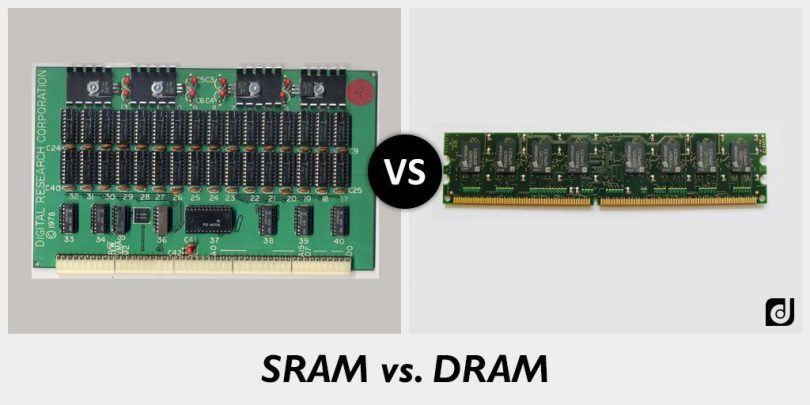
\includegraphics[width=8cm]{vs.jpg}
\centering
\caption{SRAM vs DRAM}
\label{vs}
\end{figure}

Pero yendo a más a fondo, la memoria RAM se divide en dos tipos de memorias cada una con unas especificaciones distintas para realizar una tarea determinada, estas son la memoria SRAM  y memoria DRAM( ver figura \ref{vs}) \\

\textbf{DRAM}.\\
Cada una de las celdas de la memoria RAM, a nivel circuital está constituida por un transistor y un capacitor, que en conjunto realizan un proceso muy importante , el cual consiste básicamente en recargar la memoria constantemente de información, por el cual se le denomina DRAM (Dynamic Random Access Memory -Memoria de Acceso Aleatorio Dinámica).Este tipo de memoria dinámica tiene una gran ventaja económica y en capacidad de almacenamiento frente a la memoria caché, pero a su vez, estar refrescando la información a cada instante hace que sea un proceso más  lento. \cite{augusto}\\

\noindent
\textbf{SRAM}.\\
Por otra parte, existe la memoria denominada SRAM (Static Random Access Memory -Memoria de Acceso Aleatorio estática), que a diferencia de la DRAM es mucho más veloz y la información permanece por un tiempo más prolongado sin necesidad de recargarla constantemente, gracias a su circuito interno, que contiene seis transistores y otros componentes, pero como se puede observar, al estar compuesto de más elementos, ocupa más espacio en cada celda a comparación de una DRAM, por lo cual, es económicamente más costosa, y además se obtiene una menor capacidad de almacenamiento. Es por esta razón que la memoria SRAM, es la que se usa en la memoria caché.



\subsubsection{Memoria Virtual}
Después en el nivel de jerarquías la siguiente memoria es la memoria virtual, la cual es una porción del disco duro que se dedica exclusivamente a almacenar temporalmente porciones de los programas y datos que se estén ejecutando, y que ocupan espacio innecesario en algún momento determinado, es decir, que cada vez que haya algún programa ocupando mucho volumen de la memoria RAM, pero que no se está usando, la memoria virtual se encarga de "sostenerlo" hasta próximo aviso con lo cual se aumenta la disponibilidad de almacenamiento en la RAM la cual puede ser utilizada para otros procesos. \cite{augusto}

\subsubsection{Disco Duro}
El disco duro, puede ser considerado como una memoria al igual las nombradas anteriormente, de hecho este es el espacio donde se almacenan "permanentemente"(en condiciones ideales o hasta ser borrados) todos los programas, datos, software e información que contiene el computador. A diferencia de las otras memorias, el disco duro tiene la capacidad de conservar toda la información almacenada aún después de apagar el equipo, es decir, es una memoria no volátil. El disco duro tiene una gran capacidad de almacenamiento en comparación a las memorias vistas anteriormente, la búsqueda dentro de él es muy lenta, lo cual hace que sea ineficiente para ser la memoria principal de un computador. \cite{disco}


\begin{figure}[h]
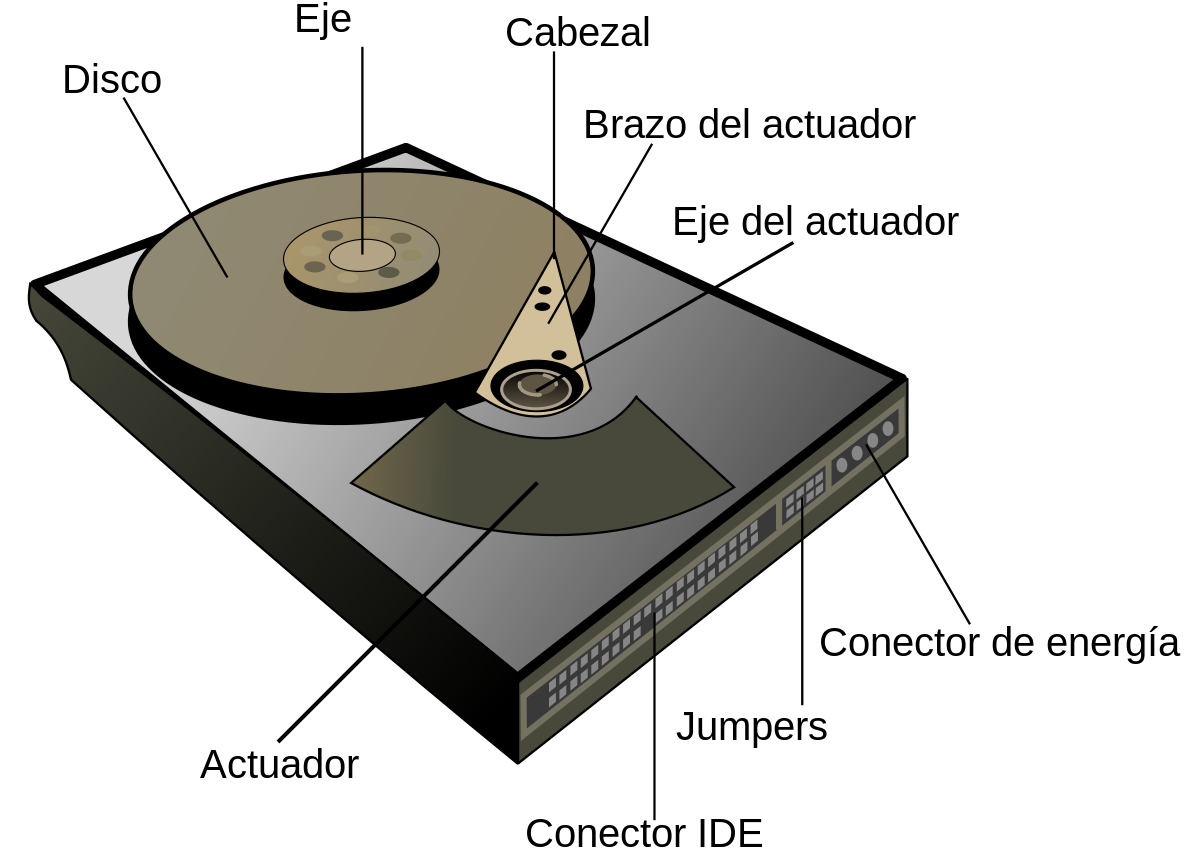
\includegraphics[width=7cm]{HDD.png}
\centering
\caption{Disco Duro}
\label{hdd}
\end{figure}

El disco duro consta de 5 partes Fundamentales para su funcionamiento(ver figura \ref{hdd}) \cite{disco}:

\begin{itemize}
    \item \textbf{Circuito impreso}:Conocido como circuito electrónico de controles, es el que se encarga de recibir las ordenes que le envía el computador, controlar  las operaciones del disco, y además de mantener la velocidad de rotación del motor constante.
    \item \textbf{Motor}:Es un motor eléctrico el cual tiene como principal función hacer girar los platos del disco.
    \item \textbf{Brazo del actuador}: Es uno de los elementos más importantes ya que se encarga de sostener los cabezales de lectura y escritura. Estos brazos se mueven usando las leyes del electromagnetismo,por lo cual puede moverse al a velocidad de la luz.
    \item \textbf{El cabezal}: Los cabezales  de lectura y escritura, son un conjunto de brazos alineados verticalmente que se mueven hacia dentro o fuera según convenga, todos a la vez. En la punta de dichos brazos están las cabezas de lectura/escritura, que gracias al movimiento del cabezal pueden leer tanto zonas interiores como exteriores del disco.
    \item \textbf{Platos}:Es aquel componente que se encarga de almacenar la información por medio de unas pistas concéntricas que se encuentran en su superficie.
\end{itemize}


\subsection{¿Cómo se gestiona la memoria en un computador?} \label{contenido}
La memoria es uno de los principales recursos de la computadora, de su correcta administración dependen las secciones de memoria de los programas que la solicitan, para ello el sistema que administra la memoria se llama administrador de memoria y su labor consiste en llevar registro de las partes de memoria que se estén utilizando y aquellas que no, con el fin de asignar espacio en memoria a los procesos cuando éstos la necesiten y liberándola cuando terminen. 
Por otra parte, la Unidad de Administración de Memoria conocida como MMU, es un dispositivo hardware que transforma las direcciones lógicas en físicas, las cuales hacen referencia a alguna posición de la memoria. El controlador de memoria envía la dirección exacta de las celdas que se desea leer o escribir y realiza la operación\cite{aragon}. Este controlador se encarga de gestionar cada tarea de la memoria interconectando las instrucciones del microprocesador y realizando la transferencia de información hacia la memoria. La memoria se encuentra conectada con su respectivo controlador a través de un bus que está ubicado en la motherBoard, estos buses son las pistas por las cuales se transporta toda la información.
A pesar de que hoy en día hay sistemas de cómputo que cuentan con una alta capacidad de memoria, es importante tener en cuenta la gestión de esta ya que hay aplicaciones que tienes más requerimientos, lo que sigue genera escasez de memoria en los sistemas multitarea y/o multiusuario.\cite{augusto} \cite{manizales}


\subsection{¿Qué hace que una memoria sea más rápida que otra? ¿Por qué esto es importante?}.\label{comparacion}
Como se pudo observar en el literal \ref{tipos}, se habló de jerarquía de memorias, donde se especifica que unas son más rápidas que otras, esto se debe a varios factores que tienen que ver tanto con la parte física de los circuitos, la arquitectura, y la frecuencia con la que funciona cada bus, por ejemplo en el caso del disco duro, al obtener tanta información y al tener una arquitectura de disco magnético, el debe dar toda la vuelta para buscar algo concreto, mientras que en la RAM al estar divida por celdas la información se obtiene de manera inmediata, además, en el caso de la memoria RAM al tener menos información es más sencillo realizar la búsqueda.\\

Por otra parte La memoria SRAM, al funcionar en sincronía con los ciclos de reloj del bus de la motherboard(placa madre), es dependiente de la frecuencia y latencia que se tenga en el sistema. Los cuales están relacionados con la siguiente expresión ( Ecuacion \ref{eq}): \\\\


\begin{equation}
\frac{Latencia(CAS)}{Frecuencia(MT/s)}*2*1024 
\label{eq}
\end{equation}
\\\\
Para finalizar, la diferencia de velocidades entre memorias es importante, porque gracias a esto se logra obtener una buena gestión y un buen equilibrio entre velocidad y almacenamiento, ya que el realizar una sola memoria que tenga una velocidad y capacidad muy grande, además de ser un proceso bastante costoso, obtendría tamaños no tan portables, es decir se tendría que crear tarjetas madre mucho más grandes, con circuitos mucho más capaces que posean gran cantidad de buses, pistas y demás elementos, lo cual para una empresa no es para nada rentable, al día de hoy esto se puede notar un poco con el disco de estado sólido (SSD-solid state disk), que es mucho más veloz que un disco duro (HDD-Hard drive disk), pero a su vez tiene un precio más elevado por la misma cantidad de almacenamiento. Por esta razón es más viable, crear una gran gama de memorias con tareas y velocidades específicas, para que así el proceso de fabricación de un computador se pueda hacer lo más comercialmente posible.


\section{Conclusiones}\label{conclusiones}
\begin{itemize}
    \item El proceso para lograr un almacenamiento óptimo y eficiente de información dentro de un computador, requiere un trabajo arduo, largo y con mucha organización; además de un estudio colaborativo entre diferentes áreas e ingenierías, para lograr una rapidez impresionante y un excelente resultado.
    \item El conocimiento y saber acerca de cómo funcionan las memorias en un computador, hace reflexionar acerca de que tan complejo es el proceso que realizan los dispositivos digitales que usamos a diario tales como Smart TV, celulares, tabletas y computadores.
    \item A pesar de la gran cantidad de tipos de memorias que existen, todas son necesarias para lograr un equilibrio entre el costo vs beneficio.
    \item El uso correcto de todos los recursos del computador en especial la memoria, debe ser una prioridad a la hora de codificar un programa, ya que como se pudo analizar en este documento, se requiere de mucho trabajo para hacer que todo funcione lo más eficiente y rápido posible.

\end{itemize}

\newpage
\noindent
\bibliographystyle{IEEEtran}
\noindent
\bibliography{references}

\end{document}